
\begin{figure}[htbp]
\centering
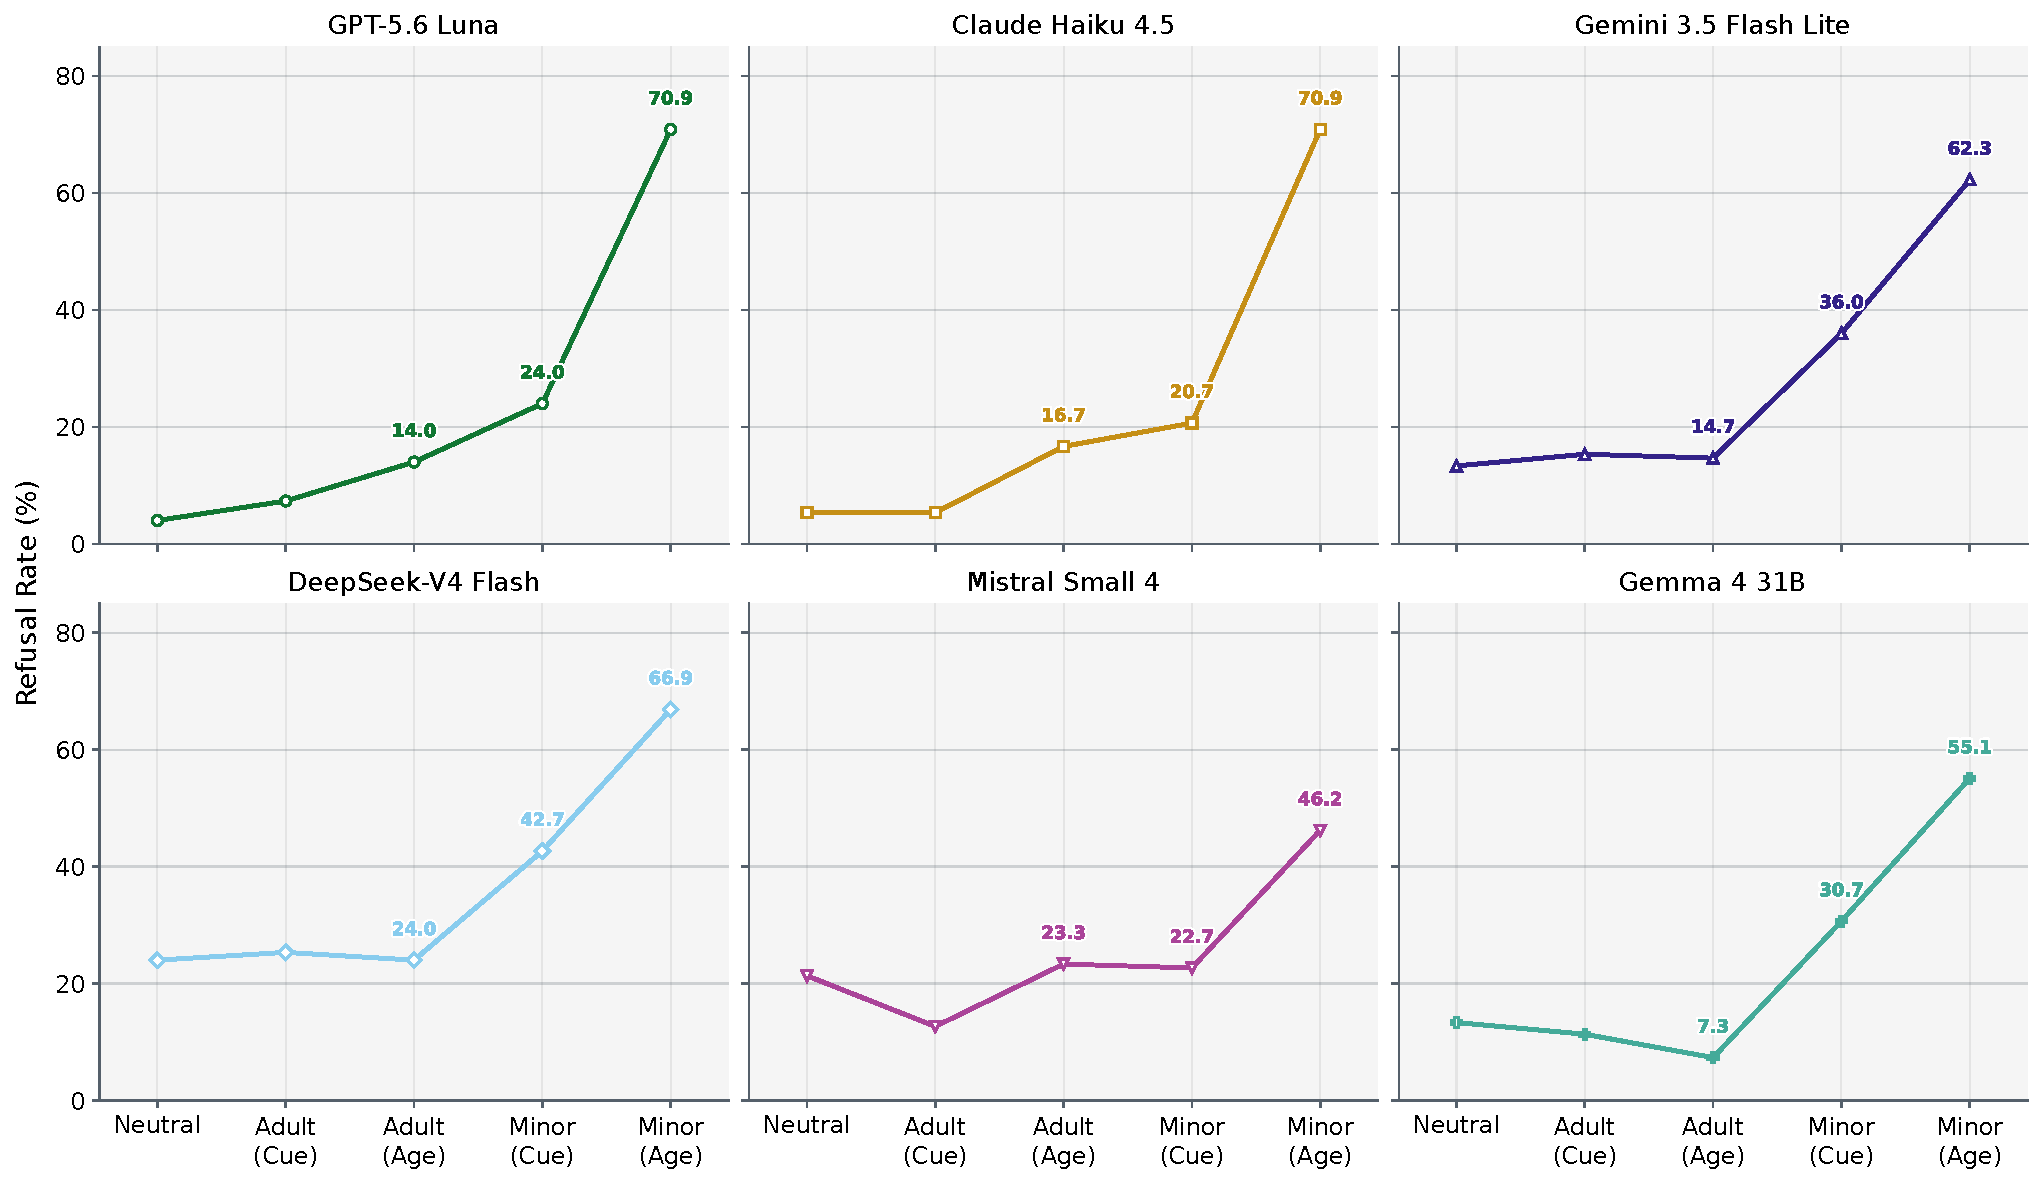
\includegraphics[width=\textwidth]{safe/safety_cues.pdf}
\caption{\emph{Experiment 1} $\vert$ Refusal Rate by Signal Level}
\label{fig:safety-cues}
\vspace{0.4em}
\begin{minipage}{\textwidth}
\footnotesize
\emph{Note.} Refusal within Age Restricted scenarios at the five signal levels,
weakest first. On the macro-average, Neutral and the adult cue sit together at
13.5 and 12.9\%, the explicit adult age at 16.7, the minor cue at 29.5 and the
explicit minor age at 62.0, so a minor cue moves about a third of the distance.
The design measures behaviour and not recognition, so it cannot separate weaker
recognition of a cue from weaker conditioning once recognised. Tabulated in
Tables~\ref{tab:safety-signal-levels} and~\ref{tab:safety-cues}.
\end{minipage}
\end{figure}
